% ============================================================
%  Information Theory --- Module 4 --- ALL DIAGRAMS (merged)
%  Compile with pdfLaTeX.  Each diagram starts on its own page.
% ============================================================
\documentclass[11pt]{article}
\usepackage[a4paper,margin=1.5cm]{geometry}
\usepackage{amsmath}
\usepackage{tikz}
\usetikzlibrary{automata,positioning,arrows.meta,trees,calc}
\usepackage{forest}
\usepackage{pgfplots}
\pgfplotsset{compat=1.18}
\setlength{\parindent}{0pt}
\title{\textbf{Information Theory --- Module 4}\\[2pt] All Diagrams (TikZ)}
\author{}
\date{}
\begin{document}
\maketitle

% ---------- Q1 : diagram 1 ----------
\clearpage
\section*{Q1 --- diagram 1}
\begin{center}
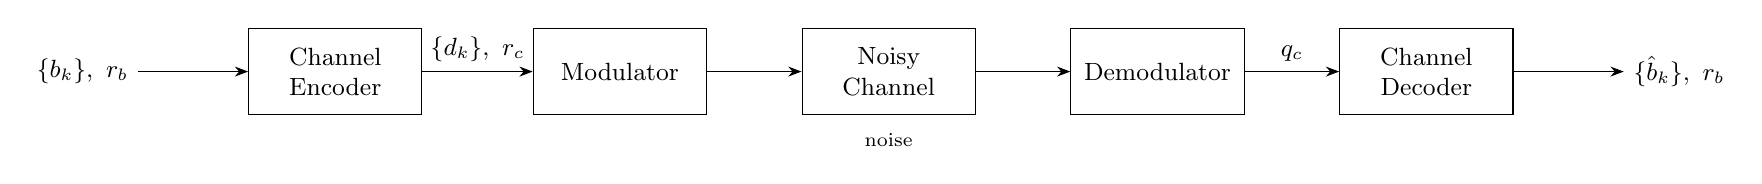
\begin{tikzpicture}[>=Stealth, font=\small,
  blk/.style={draw, minimum width=22mm, minimum height=11mm, align=center}]
  \node[blk] (enc) {Channel\\Encoder};
  \node[blk, right=14mm of enc] (mod) {Modulator};
  \node[blk, right=12mm of mod] (ch) {Noisy\\Channel};
  \node[blk, right=12mm of ch] (dem) {Demodulator};
  \node[blk, right=12mm of dem] (dec) {Channel\\Decoder};
  \draw[<-] (enc.west) -- ++(-14mm,0) node[left]{$\{b_k\},\ r_b$};
  \draw[->] (enc) -- node[above]{$\{d_k\},\ r_c$} (mod);
  \draw[->] (mod) -- (ch);
  \draw[->] (ch) -- (dem);
  \draw[->] (dem) -- node[above]{$q_c$} (dec);
  \draw[->] (dec.east) -- ++(14mm,0) node[right]{$\{\hat b_k\},\ r_b$};
  \node[below=1mm of ch, align=center, font=\scriptsize] {noise};
\end{tikzpicture}
\end{center}

% ---------- Q3 : diagram 2 ----------
\clearpage
\section*{Q3 --- diagram 2}
\begin{center}
\begin{tikzpicture}[>=Stealth, font=\small,
  xor/.style={draw,circle,inner sep=1.5pt}]
  % message bus
  \foreach \i in {1,2,3} \node (d\i) at (0,-\i*0.9) {$d_{\i}$};
  \node at (0,-3.6) {$\vdots$};
  \node (dk) at (0,-4.5) {$d_k$};
  % straight-through message outputs
  \foreach \i/\c in {1/1,2/2,3/3} \draw[->] (d\i) -- ++(7,0) node[right]{$C_{\c}=d_{\i}$};
  \draw[->] (dk) -- ++(7,0) node[right]{$C_k=d_k$};
  % check-bit adders
  \node[xor] (p1) at (4,-5.6) {$+$};
  \node[xor] (p2) at (5,-6.4) {$+$};
  \draw[->] (p1) -- ++(3,0) node[right]{$C_{k+1}$};
  \draw[->] (p2) -- ++(2,0) node[right]{$C_{n}$};
  \node at (4.5,-7.1) {\scriptsize (each $C_{k+j}=\sum_i P_{ij}d_i$, mod-2)};
\end{tikzpicture}
\end{center}

% ---------- Q4 : diagram 3 ----------
\clearpage
\section*{Q4 --- diagram 3}
\begin{center}
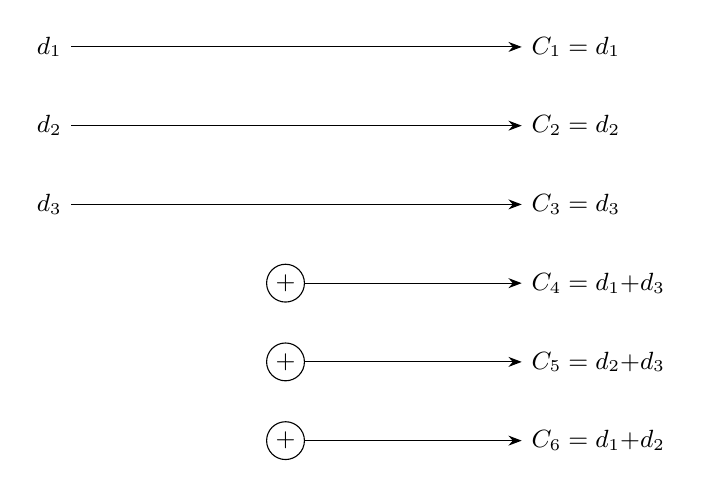
\begin{tikzpicture}[>=Stealth, font=\small, xor/.style={draw,circle,inner sep=1.5pt}]
  \node (d1) at (0,0) {$d_1$};
  \node (d2) at (0,-1) {$d_2$};
  \node (d3) at (0,-2) {$d_3$};
  \draw[->] (d1) -- ++(6,0) node[right]{$C_1=d_1$};
  \draw[->] (d2) -- ++(6,0) node[right]{$C_2=d_2$};
  \draw[->] (d3) -- ++(6,0) node[right]{$C_3=d_3$};
  \node[xor] (a4) at (3,-3) {$+$}; \draw[->] (a4)--++(3,0) node[right]{$C_4=d_1{+}d_3$};
  \node[xor] (a5) at (3,-4) {$+$}; \draw[->] (a5)--++(3,0) node[right]{$C_5=d_2{+}d_3$};
  \node[xor] (a6) at (3,-5) {$+$}; \draw[->] (a6)--++(3,0) node[right]{$C_6=d_1{+}d_2$};
\end{tikzpicture}
\end{center}

% ---------- Q4 : diagram 4 ----------
\clearpage
\section*{Q4 --- diagram 4}
\begin{center}
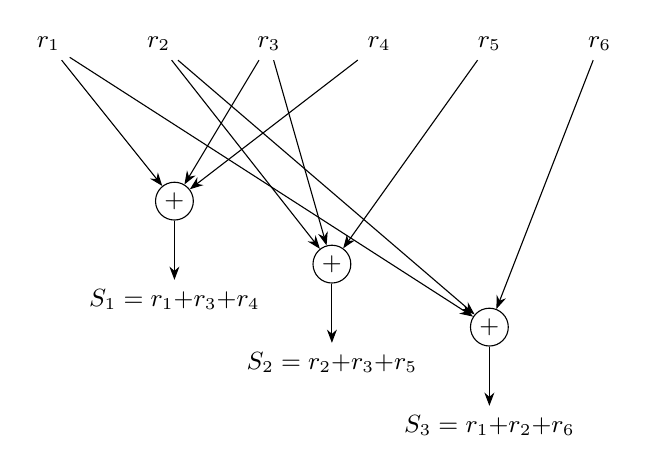
\begin{tikzpicture}[>=Stealth, font=\small, xor/.style={draw,circle,inner sep=1.5pt}]
  \foreach \i in {1,...,6}\node (r\i) at (\i*1.4,0) {$r_{\i}$};
  \node[xor] (s1) at (3,-2) {$+$}; \draw[->](s1)--++(0,-1) node[below]{$S_1=r_1{+}r_3{+}r_4$};
  \node[xor] (s2) at (5,-2.8){$+$}; \draw[->](s2)--++(0,-1) node[below]{$S_2=r_2{+}r_3{+}r_5$};
  \node[xor] (s3) at (7,-3.6){$+$}; \draw[->](s3)--++(0,-1) node[below]{$S_3=r_1{+}r_2{+}r_6$};
  \draw[->](r1)--(s1); \draw[->](r3)--(s1); \draw[->](r4)--(s1);
  \draw[->](r2)--(s2); \draw[->](r3)--(s2); \draw[->](r5)--(s2);
  \draw[->](r1)--(s3); \draw[->](r2)--(s3); \draw[->](r6)--(s3);
\end{tikzpicture}
\end{center}

% ---------- Q8 : diagram 5 ----------
\clearpage
\section*{Q8 --- diagram 5}
\begin{center}
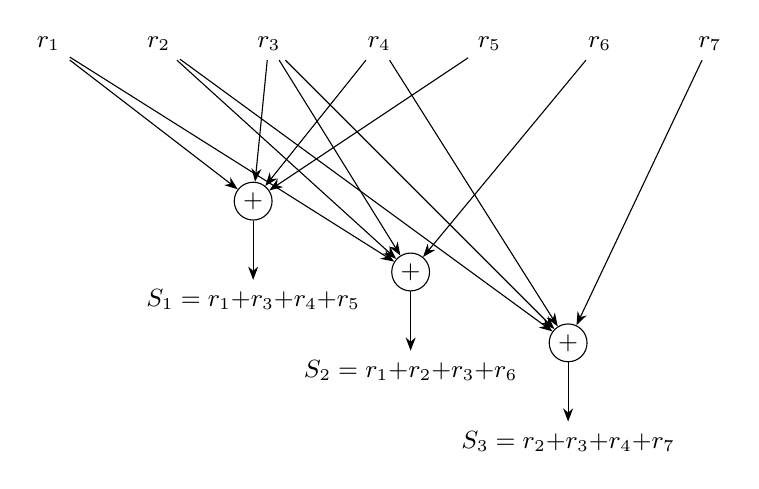
\begin{tikzpicture}[>=Stealth, font=\small, xor/.style={draw,circle,inner sep=1.5pt}]
  \foreach \i in {1,...,7}\node (r\i) at (\i*1.4,0){$r_{\i}$};
  \node[xor] (s1) at (4,-2)  {$+$}; \draw[->](s1)--++(0,-1) node[below]{$S_1=r_1{+}r_3{+}r_4{+}r_5$};
  \node[xor] (s2) at (6,-2.9){$+$}; \draw[->](s2)--++(0,-1) node[below]{$S_2=r_1{+}r_2{+}r_3{+}r_6$};
  \node[xor] (s3) at (8,-3.8){$+$}; \draw[->](s3)--++(0,-1) node[below]{$S_3=r_2{+}r_3{+}r_4{+}r_7$};
  \draw[->](r1)--(s1);\draw[->](r3)--(s1);\draw[->](r4)--(s1);\draw[->](r5)--(s1);
  \draw[->](r1)--(s2);\draw[->](r2)--(s2);\draw[->](r3)--(s2);\draw[->](r6)--(s2);
  \draw[->](r2)--(s3);\draw[->](r3)--(s3);\draw[->](r4)--(s3);\draw[->](r7)--(s3);
\end{tikzpicture}
\end{center}

% ---------- Q10 : diagram 6 ----------
\clearpage
\section*{Q10 --- diagram 6}
\begin{center}
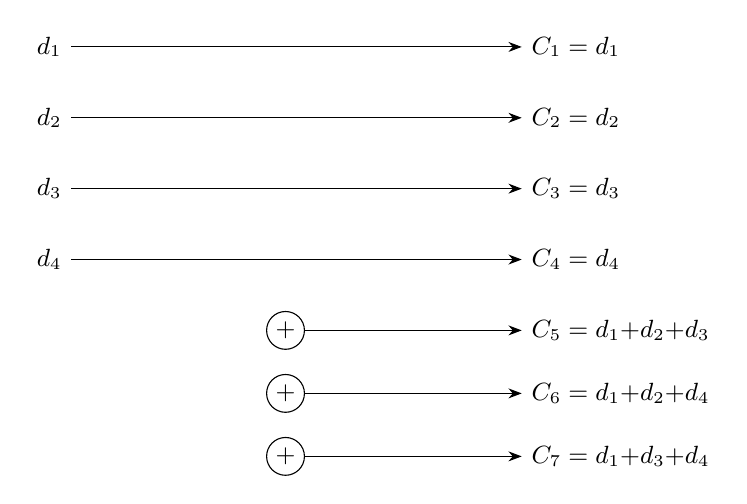
\begin{tikzpicture}[>=Stealth, font=\small, xor/.style={draw,circle,inner sep=1.5pt}]
  \foreach \i in {1,2,3,4}\node (d\i) at (0,-\i*0.9){$d_{\i}$};
  \foreach \i in {1,2,3,4}\draw[->](d\i)--++(6,0) node[right]{$C_{\i}=d_{\i}$};
  \node[xor](c5) at (3,-4.5){$+$}; \draw[->](c5)--++(3,0) node[right]{$C_5=d_1{+}d_2{+}d_3$};
  \node[xor](c6) at (3,-5.3){$+$}; \draw[->](c6)--++(3,0) node[right]{$C_6=d_1{+}d_2{+}d_4$};
  \node[xor](c7) at (3,-6.1){$+$}; \draw[->](c7)--++(3,0) node[right]{$C_7=d_1{+}d_3{+}d_4$};
\end{tikzpicture}
\end{center}

% ---------- Q10 : diagram 7 ----------
\clearpage
\section*{Q10 --- diagram 7}
\begin{center}
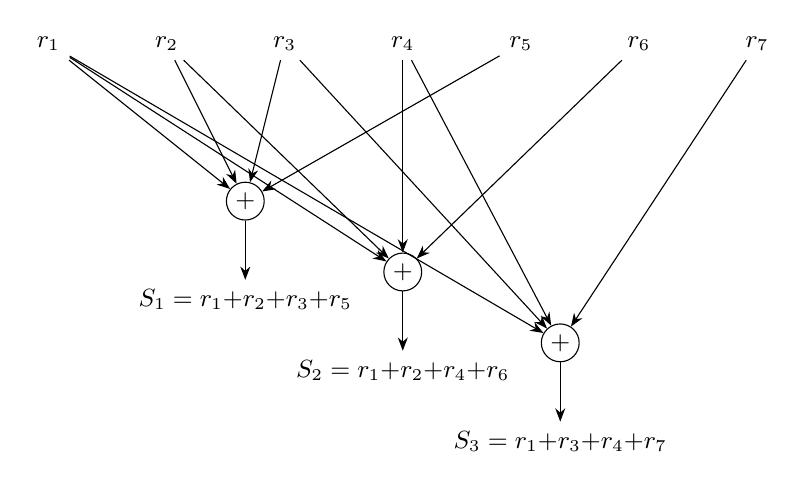
\begin{tikzpicture}[>=Stealth, font=\small, xor/.style={draw,circle,inner sep=1.5pt}]
  \foreach \i in {1,...,7}\node (r\i) at (\i*1.5,0){$r_{\i}$};
  \node[xor](s1) at (4,-2)  {$+$}; \draw[->](s1)--++(0,-1) node[below]{$S_1=r_1{+}r_2{+}r_3{+}r_5$};
  \node[xor](s2) at (6,-2.9){$+$}; \draw[->](s2)--++(0,-1) node[below]{$S_2=r_1{+}r_2{+}r_4{+}r_6$};
  \node[xor](s3) at (8,-3.8){$+$}; \draw[->](s3)--++(0,-1) node[below]{$S_3=r_1{+}r_3{+}r_4{+}r_7$};
  \draw[->](r1)--(s1);\draw[->](r2)--(s1);\draw[->](r3)--(s1);\draw[->](r5)--(s1);
  \draw[->](r1)--(s2);\draw[->](r2)--(s2);\draw[->](r4)--(s2);\draw[->](r6)--(s2);
  \draw[->](r1)--(s3);\draw[->](r3)--(s3);\draw[->](r4)--(s3);\draw[->](r7)--(s3);
\end{tikzpicture}
\end{center}

% ---------- Q12 : diagram 8 ----------
\clearpage
\section*{Q12 --- diagram 8}
\begin{center}
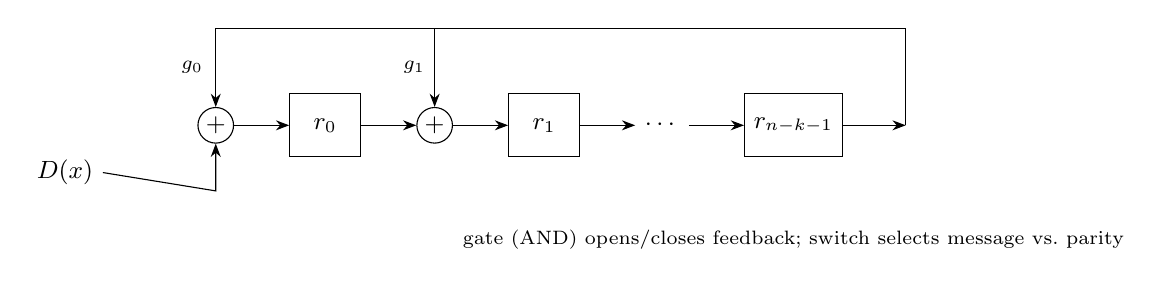
\begin{tikzpicture}[>=Stealth, font=\small,
  ff/.style={draw,minimum width=9mm,minimum height=8mm},
  add/.style={draw,circle,inner sep=1.2pt}]
  \node[add](a0){$+$};
  \node[ff,right=7mm of a0](r0){$r_0$};
  \node[add,right=7mm of r0](a1){$+$};
  \node[ff,right=7mm of a1](r1){$r_1$};
  \node[right=7mm of r1](dots){$\cdots$};
  \node[ff,right=7mm of dots](rl){$r_{n-k-1}$};
  \draw[->](a0)--(r0); \draw[->](r0)--(a1); \draw[->](a1)--(r1);
  \draw[->](r1)--(dots); \draw[->](dots)--(rl);
  % feedback bus along the top
  \coordinate (out) at ($(rl.east)+(8mm,0)$);
  \draw[->](rl.east)--(out);
  \draw (out)|-($(a0.north)+(0,10mm)$);
  \draw[->]($(a0.north)+(0,10mm)$)-|(a0.north);
  \draw[->]($(a1.north)+(0,10mm)$)-- node[left]{\scriptsize $g_1$} (a1.north);
  \node at ($(a0.north)+(-3mm,5mm)$){\scriptsize $g_0$};
  % message input switch
  \draw[->]($(a0.west)+(-12mm,-6mm)$) node[left]{$D(x)$} -- ($(a0.south)+(0,-6mm)$) -- (a0.south);
  \node[below=8mm of rl]{\scriptsize gate (AND) opens/closes feedback; switch selects message vs.\ parity};
\end{tikzpicture}
\end{center}

% ---------- Q13 : diagram 9 ----------
\clearpage
\section*{Q13 --- diagram 9}
\begin{center}
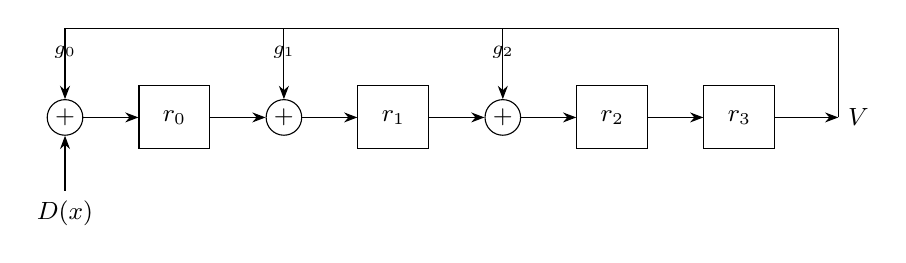
\begin{tikzpicture}[>=Stealth, font=\small,
  ff/.style={draw,minimum width=9mm,minimum height=8mm}, add/.style={draw,circle,inner sep=1.2pt}]
  \node[add](a0){$+$};
  \node[ff,right=7mm of a0](r0){$r_0$};
  \node[add,right=7mm of r0](a1){$+$};
  \node[ff,right=7mm of a1](r1){$r_1$};
  \node[add,right=7mm of r1](a2){$+$};
  \node[ff,right=7mm of a2](r2){$r_2$};
  \node[ff,right=7mm of r2](r3){$r_3$};
  \draw[->](a0)--(r0);\draw[->](r0)--(a1);\draw[->](a1)--(r1);
  \draw[->](r1)--(a2);\draw[->](a2)--(r2);\draw[->](r2)--(r3);
  \coordinate(out) at ($(r3.east)+(8mm,0)$); \draw[->](r3.east)--(out) node[right]{$V$};
  \draw (out)|-($(a0.north)+(0,9mm)$);
  \draw[->]($(a0.north)+(0,9mm)$)-|(a0.north);
  \draw[->]($(a1.north)+(0,9mm)$)--(a1.north);
  \draw[->]($(a2.north)+(0,9mm)$)--(a2.north);
  \node[font=\scriptsize] at ($(a0.north)+(0,6mm)$){$g_0$};
  \node[font=\scriptsize] at ($(a1.north)+(0,6mm)$){$g_1$};
  \node[font=\scriptsize] at ($(a2.north)+(0,6mm)$){$g_2$};
  \draw[->]($(a0.south)+(0,-7mm)$) node[below]{$D(x)$} -- (a0.south);
\end{tikzpicture}
\end{center}

% ---------- Q14 : diagram 10 ----------
\clearpage
\section*{Q14 --- diagram 10}
\begin{center}
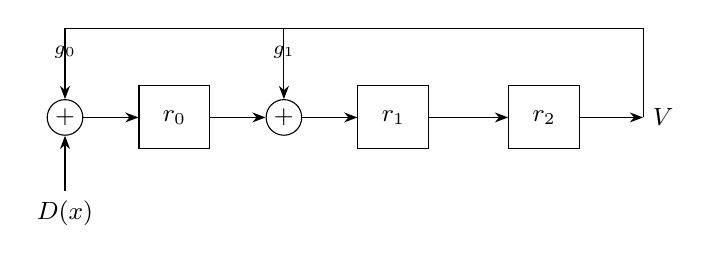
\begin{tikzpicture}[>=Stealth, font=\small,
  ff/.style={draw,minimum width=9mm,minimum height=8mm}, add/.style={draw,circle,inner sep=1.2pt}]
  \node[add](a0){$+$};
  \node[ff,right=7mm of a0](r0){$r_0$};
  \node[add,right=7mm of r0](a1){$+$};
  \node[ff,right=7mm of a1](r1){$r_1$};
  \node[ff,right=10mm of r1](r2){$r_2$};
  \draw[->](a0)--(r0);\draw[->](r0)--(a1);\draw[->](a1)--(r1);\draw[->](r1)--(r2);
  \coordinate(out) at ($(r2.east)+(8mm,0)$); \draw[->](r2.east)--(out) node[right]{$V$};
  \draw (out)|-($(a0.north)+(0,9mm)$);
  \draw[->]($(a0.north)+(0,9mm)$)-|(a0.north);
  \draw[->]($(a1.north)+(0,9mm)$)--(a1.north);
  \node[font=\scriptsize] at ($(a0.north)+(0,6mm)$){$g_0$};
  \node[font=\scriptsize] at ($(a1.north)+(0,6mm)$){$g_1$};
  \draw[->]($(a0.south)+(0,-7mm)$) node[below]{$D(x)$} -- (a0.south);
\end{tikzpicture}
\end{center}

% ---------- Q15 : diagram 11 ----------
\clearpage
\section*{Q15 --- diagram 11}
\begin{center}
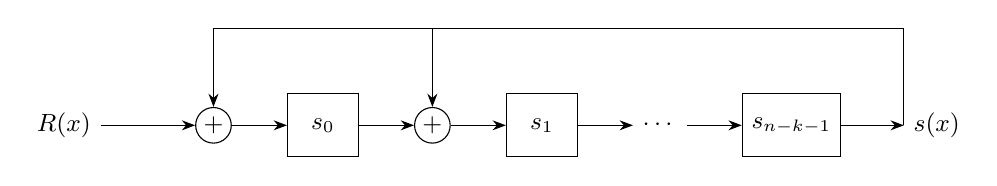
\begin{tikzpicture}[>=Stealth, font=\small,
  ff/.style={draw,minimum width=9mm,minimum height=8mm}, add/.style={draw,circle,inner sep=1.2pt}]
  \node[add](a0){$+$};
  \node[ff,right=7mm of a0](s0){$s_0$};
  \node[add,right=7mm of s0](a1){$+$};
  \node[ff,right=7mm of a1](s1){$s_1$};
  \node[right=7mm of s1](dots){$\cdots$};
  \node[ff,right=7mm of dots](sl){$s_{n-k-1}$};
  \draw[->](a0)--(s0);\draw[->](s0)--(a1);\draw[->](a1)--(s1);
  \draw[->](s1)--(dots);\draw[->](dots)--(sl);
  \draw[->]($(a0.west)+(-12mm,0)$) node[left]{$R(x)$} -- (a0.west);
  \coordinate(out) at ($(sl.east)+(8mm,0)$); \draw[->](sl.east)--(out) node[right]{$s(x)$};
  \draw (out)|-($(a0.north)+(0,10mm)$);
  \draw[->]($(a0.north)+(0,10mm)$)-|(a0.north);
  \draw[->]($(a1.north)+(0,10mm)$)--(a1.north);
\end{tikzpicture}
\end{center}

% ---------- Q17 : diagram 12 ----------
\clearpage
\section*{Q17 --- diagram 12}
\begin{center}
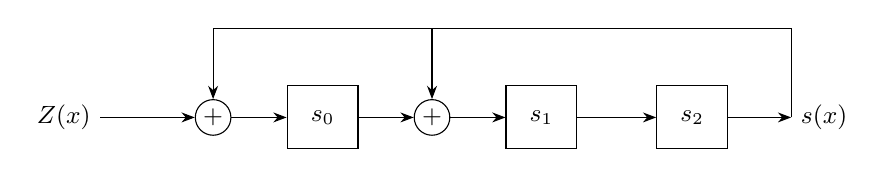
\begin{tikzpicture}[>=Stealth, font=\small,
  ff/.style={draw,minimum width=9mm,minimum height=8mm}, add/.style={draw,circle,inner sep=1.2pt}]
  \node[add](a0){$+$};
  \node[ff,right=7mm of a0](s0){$s_0$};
  \node[add,right=7mm of s0](a1){$+$};
  \node[ff,right=7mm of a1](s1){$s_1$};
  \node[ff,right=10mm of s1](s2){$s_2$};
  \draw[->](a0)--(s0);\draw[->](s0)--(a1);\draw[->](a1)--(s1);\draw[->](s1)--(s2);
  \draw[->]($(a0.west)+(-12mm,0)$) node[left]{$Z(x)$} -- (a0.west);
  \coordinate(out) at ($(s2.east)+(8mm,0)$); \draw[->](s2.east)--(out) node[right]{$s(x)$};
  \draw (out)|-($(a0.north)+(0,9mm)$);
  \draw[->]($(a0.north)+(0,9mm)$)-|(a0.north);
  \draw[->]($(a1.north)+(0,9mm)$)--(a1.north);
\end{tikzpicture}
\end{center}

% ---------- Q18 : diagram 13 ----------
\clearpage
\section*{Q18 --- diagram 13}
\begin{center}
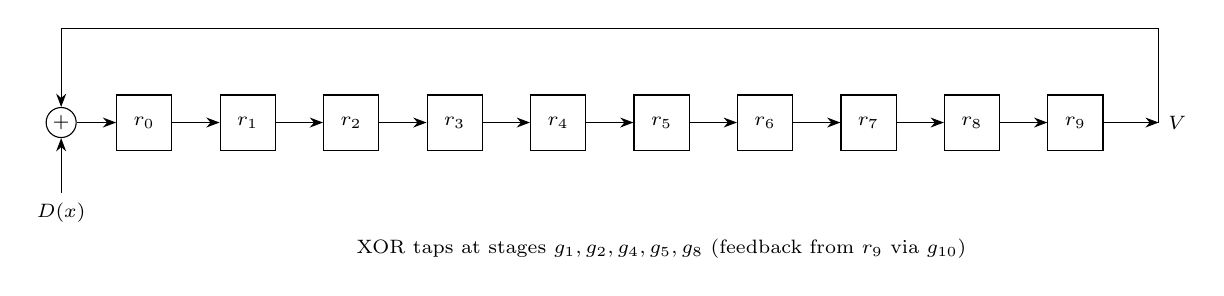
\begin{tikzpicture}[>=Stealth, font=\scriptsize,
  ff/.style={draw,minimum width=7mm,minimum height=7mm}, add/.style={draw,circle,inner sep=1pt}]
  \node[add](a0){$+$};
  \foreach \i [remember=\i as \p (initially 0)] in {0,...,9}{
     \ifnum\i=0 \node[ff,right=5mm of a0](r0){$r_0$};
     \else \node[ff,right=6mm of r\p](r\i){$r_\i$}; \fi }
  % taps (XOR) before stages where g_i=1 for i=1,2,4,5,8 (g0 at a0, g10 feedback)
  \draw[->](a0)--(r0);
  \foreach \i [remember=\i as \p (initially 0)] in {1,...,9}{ \draw[->](r\p)--(r\i); }
  \coordinate(out) at ($(r9.east)+(7mm,0)$); \draw[->](r9.east)--(out) node[right]{$V$};
  \draw (out)|-($(a0.north)+(0,10mm)$); \draw[->]($(a0.north)+(0,10mm)$)-|(a0.north);
  \draw[->]($(a0.south)+(0,-7mm)$) node[below]{$D(x)$}--(a0.south);
  \node[align=center,below=10mm of r5]{\scriptsize XOR taps at stages $g_1,g_2,g_4,g_5,g_8$ (feedback from $r_9$ via $g_{10}$)};
\end{tikzpicture}
\end{center}

% ---------- Q19 : diagram 14 ----------
\clearpage
\section*{Q19 --- diagram 14}
\begin{center}
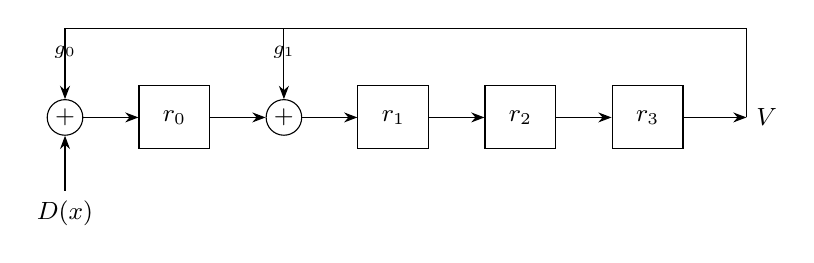
\begin{tikzpicture}[>=Stealth, font=\small,
  ff/.style={draw,minimum width=9mm,minimum height=8mm}, add/.style={draw,circle,inner sep=1.2pt}]
  \node[add](a0){$+$};
  \node[ff,right=7mm of a0](r0){$r_0$};
  \node[add,right=7mm of r0](a1){$+$};
  \node[ff,right=7mm of a1](r1){$r_1$};
  \node[ff,right=7mm of r1](r2){$r_2$};
  \node[ff,right=7mm of r2](r3){$r_3$};
  \draw[->](a0)--(r0);\draw[->](r0)--(a1);\draw[->](a1)--(r1);\draw[->](r1)--(r2);\draw[->](r2)--(r3);
  \coordinate(out) at ($(r3.east)+(8mm,0)$); \draw[->](r3.east)--(out) node[right]{$V$};
  \draw (out)|-($(a0.north)+(0,9mm)$); \draw[->]($(a0.north)+(0,9mm)$)-|(a0.north);
  \draw[->]($(a1.north)+(0,9mm)$)--(a1.north);
  \node[font=\scriptsize] at ($(a0.north)+(0,6mm)$){$g_0$};
  \node[font=\scriptsize] at ($(a1.north)+(0,6mm)$){$g_1$};
  \draw[->]($(a0.south)+(0,-7mm)$) node[below]{$D(x)$}--(a0.south);
\end{tikzpicture}
\end{center}

% ---------- Q20 : diagram 15 ----------
\clearpage
\section*{Q20 --- diagram 15}
\begin{center}
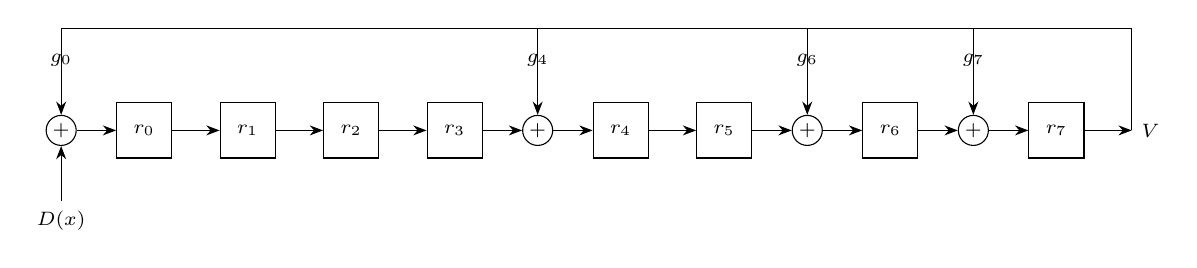
\begin{tikzpicture}[>=Stealth, font=\scriptsize,
  ff/.style={draw,minimum width=7mm,minimum height=7mm}, add/.style={draw,circle,inner sep=1pt}]
  \node[add](a0){$+$};
  \node[ff,right=5mm of a0](r0){$r_0$};
  \node[ff,right=6mm of r0](r1){$r_1$};
  \node[ff,right=6mm of r1](r2){$r_2$};
  \node[ff,right=6mm of r2](r3){$r_3$};
  \node[add,right=5mm of r3](a4){$+$};
  \node[ff,right=5mm of a4](r4){$r_4$};
  \node[ff,right=6mm of r4](r5){$r_5$};
  \node[add,right=5mm of r5](a6){$+$};
  \node[ff,right=5mm of a6](r6){$r_6$};
  \node[add,right=5mm of r6](a7){$+$};
  \node[ff,right=5mm of a7](r7){$r_7$};
  \draw[->](a0)--(r0);\draw[->](r0)--(r1);\draw[->](r1)--(r2);\draw[->](r2)--(r3);
  \draw[->](r3)--(a4);\draw[->](a4)--(r4);\draw[->](r4)--(r5);\draw[->](r5)--(a6);
  \draw[->](a6)--(r6);\draw[->](r6)--(a7);\draw[->](a7)--(r7);
  \coordinate(out) at ($(r7.east)+(6mm,0)$); \draw[->](r7.east)--(out) node[right]{$V$};
  \draw (out)|-($(a0.north)+(0,11mm)$); \draw[->]($(a0.north)+(0,11mm)$)-|(a0.north);
  \draw[->]($(a4.north)+(0,11mm)$)--(a4.north);
  \draw[->]($(a6.north)+(0,11mm)$)--(a6.north);
  \draw[->]($(a7.north)+(0,11mm)$)--(a7.north);
  \node at ($(a0.north)+(0,7mm)$){$g_0$};\node at ($(a4.north)+(0,7mm)$){$g_4$};
  \node at ($(a6.north)+(0,7mm)$){$g_6$};\node at ($(a7.north)+(0,7mm)$){$g_7$};
  \draw[->]($(a0.south)+(0,-7mm)$) node[below]{$D(x)$}--(a0.south);
\end{tikzpicture}
\end{center}
\end{document}
